%\ifthenelse{\boolean{arxiv}}{
\begin{figure*}[t]
    \centering
    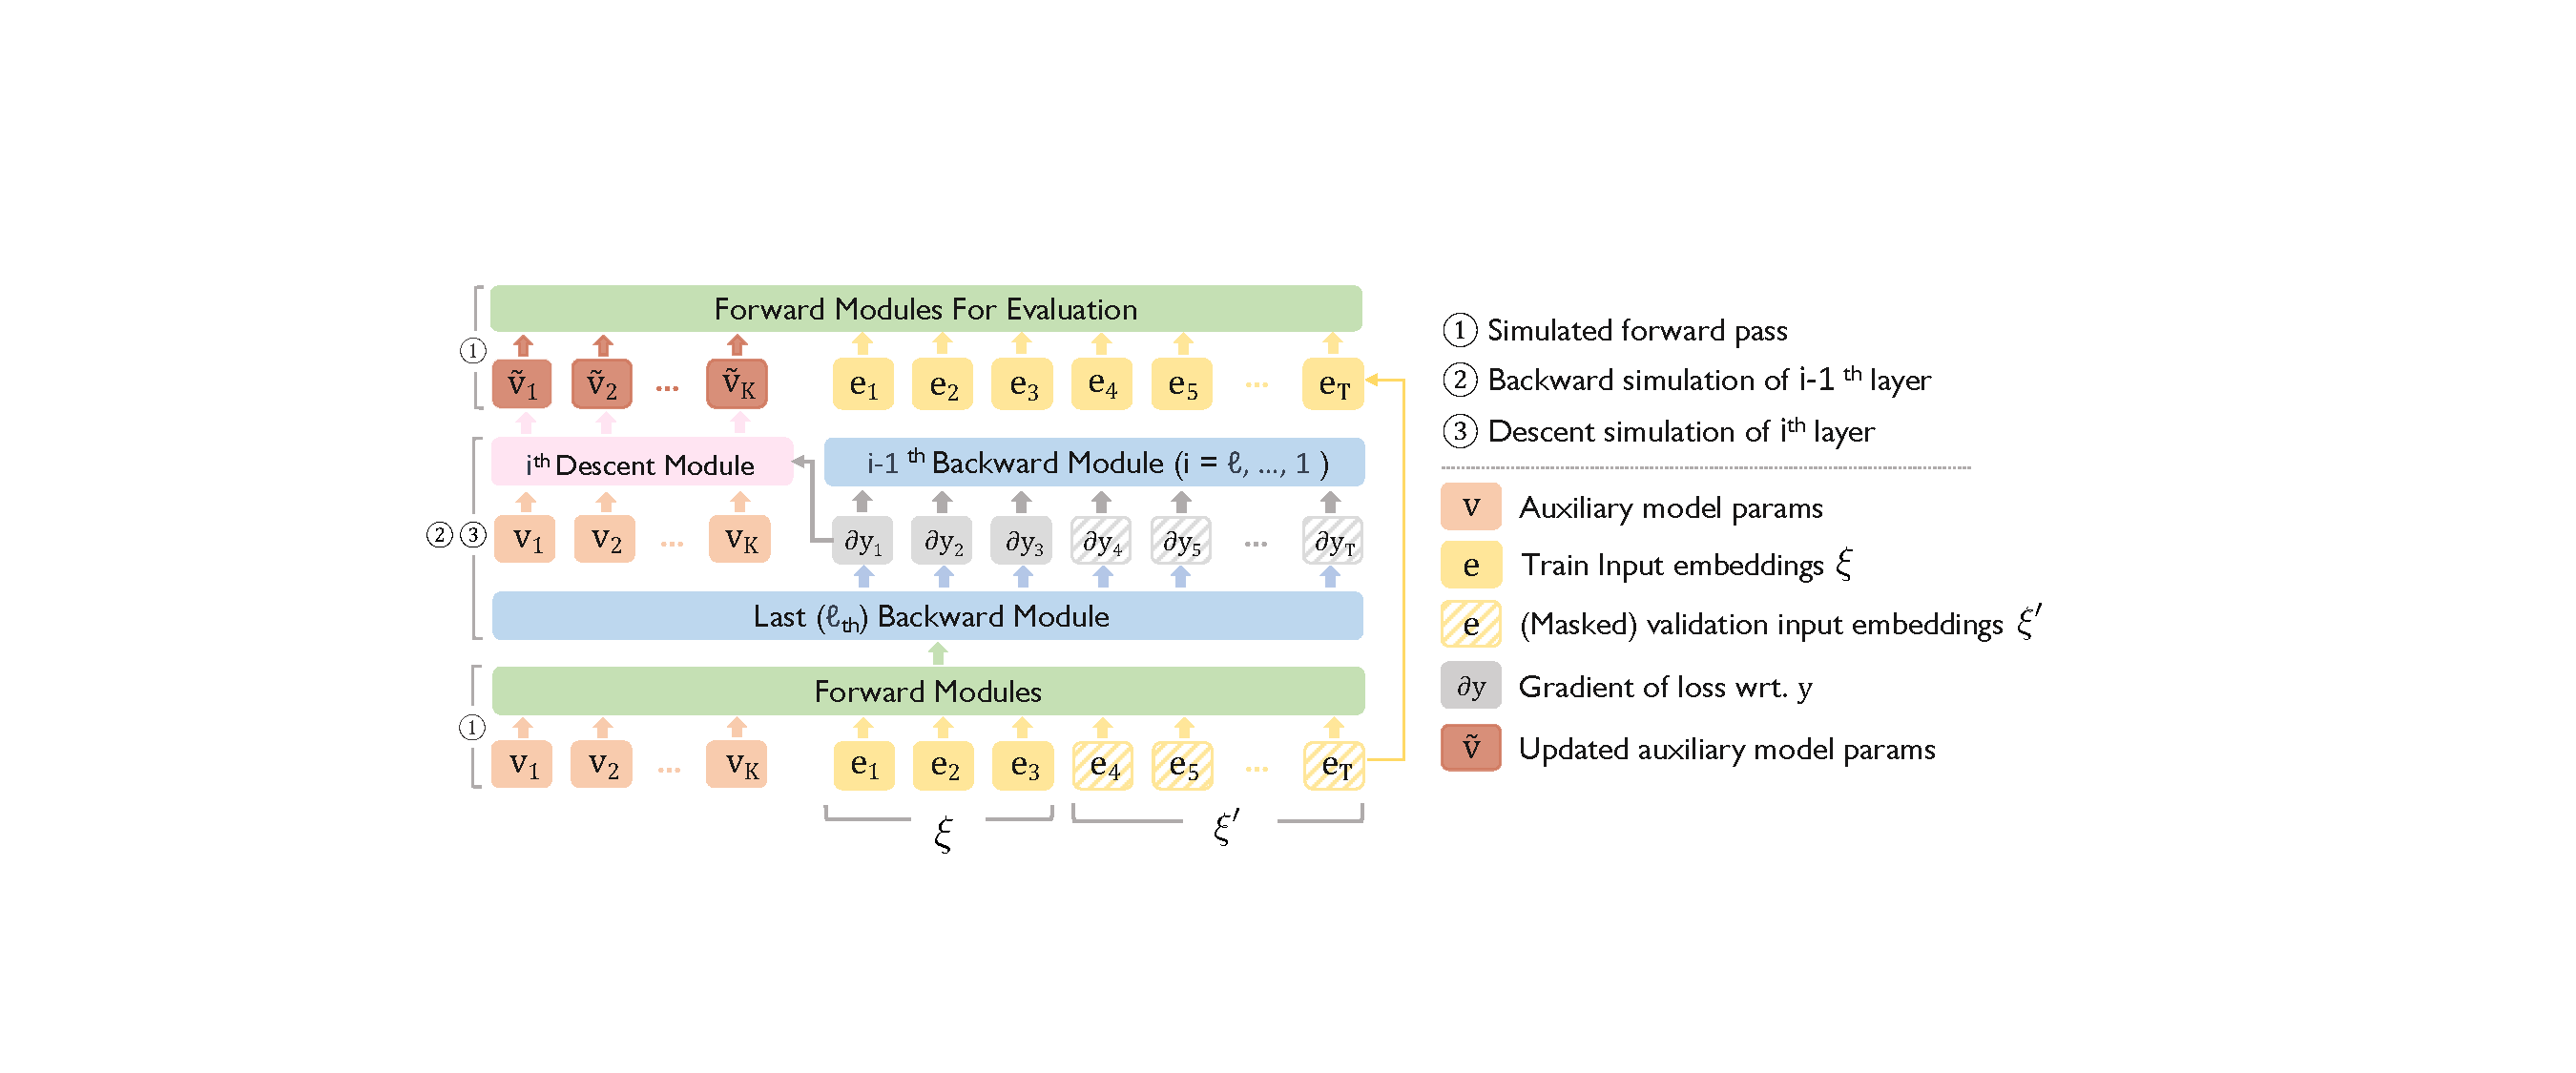
\includegraphics[width=\textwidth]{figures/Final_images.pdf}
    \caption{The overall structure of \textsc{TinT} (see~\Cref{sec:design} for an overview). Each forward, backward, and descent module is represented using combinations of linear, self-attention, layernorm, and activation layers.
    The input consists of prefix embeddings (\Cref{def:prefix_embs}) that represent relevant auxiliary model parameters in each layer followed by natural language input. A prefix mask separates the train and test segments of the input (\textsection\ref{sec:input_structure}). 
    %Auxiliary model parameters are updated in the descent module using the training part, and the updated prefix tokens are transferred to the forward modules via residual connections for evaluating the rest. 
    %\snote{Update figure to contain $\xi$ and $\xi'$ notation.}
    }
    \label{fig:general_structure_simulator}
\end{figure*}
%}{

\iffalse
\begin{figure}
    \centering
    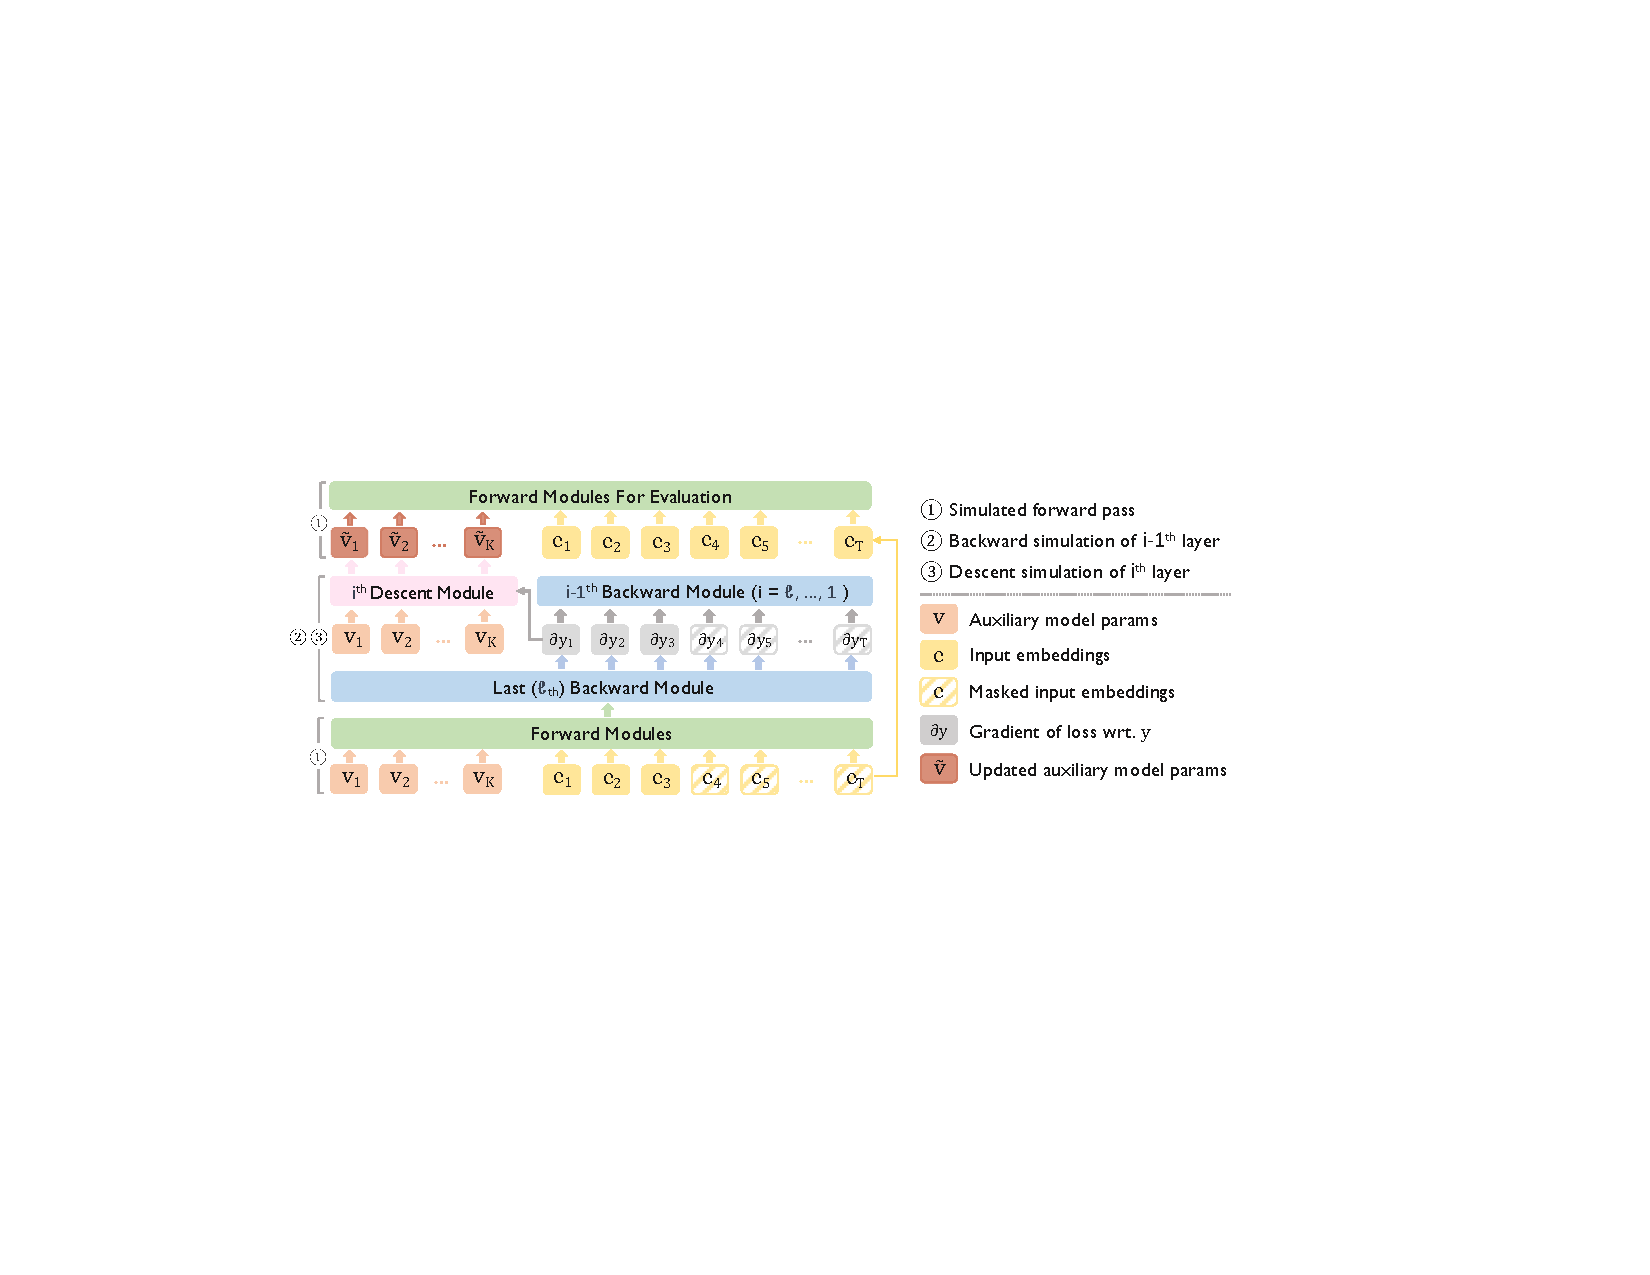
\includegraphics[width=\textwidth]{figures/figure1.pdf}
    \caption{The overall structure of \textsc{TinT}. The input consists of prefix embeddings, that represent relevant auxiliary model parameters in each layer, input token embeddings, and a binary prefix mask to separate the train and evaluation segments of the input. The auxiliary model parameters are updated in the descent module using the training part of the segment, and the updated prefix tokens are transferred to the forward modules via residual connections for evaluating the rest of the segment. 
    }
\end{figure}
}
\fi